% introduction.tex

\section{Introduction}
Voldemort is an implementation of a distributed, highly available key-value store.
The configuration of the system is however cumbersome and tedious, so we would like to explore the possibilities for using ZooKeeper to coordinate configuration and later some management tasks.
Such tasks includes extending and reducing the members of the cluster.

We have created a method for managing cluster metadata and configuration for Voldemort by using Apache ZooKeeper for coordination.

In this process we have implemented an internal StorageEngine that uses ZooKeeper for node configuration and metadata.

We have also implemented a service, named Headmaster, that manages configuration, node discovery and node membership in the cluster.
Headmaster can also decide whether to execute a rebalance based on certain criteria.

\subsection{Voldemort and Dynamo}
Voldemort is a software system based off of Amazon's paper on Dynamo, Amazon's highly available key-value store\cite{dynamo}.

The supported queries are limited to simple get and put operations on objects uniquely identified by a key. 
The objects stored are by the system considered binary blobs.
The database is mainly used to store lots of smaller items, typically less than 1MB in size.

\subsubsection{Motivation for these systems}
Traditional relational database systems are generally very safe to use, usually providing all of the ACID (\emph{Atomicity, Consistency, Isolation, Durability}) properties.
This guarantees that all committed transactions are processed reliably.
Experience has however shown that databases providing ACID guarantees have trouble scaling. It is very difficult, if not impossible, to have ACID databases handle the high traffic volumes in addition to the high availability demands of today.

Voldemort and Dynamo sacrifices consistency and isolation requirements to achieve higher availability with satisfactory durability.
In fact, we will later see that most of this behavior is easily tunable and left as design choices per implementation.
You should also note Voldemort (and Dynamo) does not guarantee any form of isolation and does not support multiple key updates.

\subsection{Techniques and technologies}
The software used in this project employ many different and important techniques known from distributed computing, and will be discussed here.

\subsubsection{PAXOS}

\subsubsection{Consistent hashing}
\label{sec:consistenthashing}
Consistent hashing is a technique introduced in 1997 by David Karger et al.\cite{Karger97consistenthashing}
The technique is used to solve problems with locating a key in a distributed system.
Let's assume you have $n$ servers in the system, then number these from $0$ to $n-1$.
The hashspace of the keys are then divided into $n$ partitions. Then do a $\textrm{Hash(key) mod } n$ and you have the server location for the key.

However, with this scheme if a server fails and you now have $n-1=m$ servers, all the failed server's data is gone.
You have to invalidate all existing servers, renumber your set of servers and start over.

Consistent hashing reduces this problem by assigning each node with a number of points in the hash space.
The hash space is viewed as a ring by wrapping around \texttt{0000-FFFF}. The nodes are placed at points along the ring as in Figure \ref{fig:hashring}. When a key is looked up, you find it's place on the ring and move clockwise to the first point with an assigned node. In Figure \ref{fig:hashring}, key K is routed to the next node on the ring, node B.

Now remember we let the nodes take on \emph{several} points along the ring, thus spreading a nodes responsible key space to smaller pieces along the ring.
I.e. nodes B, E and G in Figure \ref{fig:hashring} could be the same \emph{physical} node.

\begin{figure}[h]
    \centering
    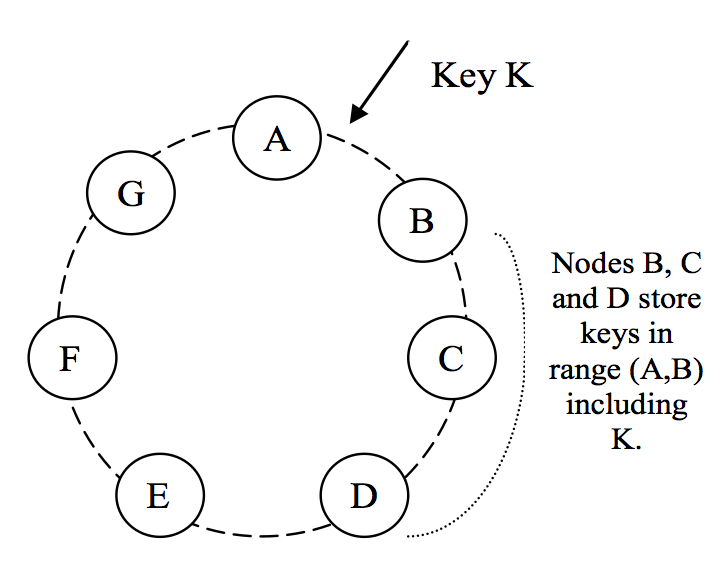
\includegraphics[width=0.5\textwidth]{introduction/hashring}
    \caption{Hash ring with several nodes\cite{dynamo}.}
    \label{fig:hashring}
\end{figure}

This approach to locating keys has several advantages:

\begin{itemize}
\item Like before, we distribute operations on the set of available servers. By having each server take numerous positions on the hash ring, we also gain a more even distribution of the amount of key space among the nodes, compared to giving them a random or fixed position.

\item Consistent hashing can also accommodate different types of servers by allowing more powerful nodes to have more points assigned on the ring, and vice versa. 

\item When adding a new server, a number of different areas around the circle are affected, and not one contiguous piece. This means the work of adding in the new node will be spread over the system, and not all requests routed to a single node.

\item The spread of the key space also avoids rehashing of more than $k/n$ keys when adding a new node. 

\item When a node fails, you move along the ring to the next server. When the nodes occupy several points on the ring, this results in the work from a failing node being distributed among all the nodes in the system.
\end{itemize}

Consistent hashing also conveniently allows for easy, tunable replication of data to ensure durability, as used by key-value stores Dynamo\cite{dynamo} and Voldemort\cite{voldemort}. Consider W the number of data replicas to create. Hash the key, then move along the ring, writing key K to the W first nodes encountered on the ring. This will also ensure backups to be available along the ring when a node fails and requests gets passed along.

\subsubsection{Durability}
As explained in \ref{sec:consistenthashing}, both Voldemort and Dynamo use consistent hashing to locate and and store keys.
They are both key-value stores only.
The goals for the Voldemort project is a database which is highly available and fault tolerant, providing an \emph{always-on} experience.

To allow for safely storing user data, redundancy is required. 
The typical approach to this is synchronously storing replicas at different locations to ensure data replication. 
In practice though, providing this kind of strong consistency in a database system can prove detrimental to availability in some failure scenarios.
A common approach to failure is locking down data and making it unavailable until the failure is resolved, so as not to serve potentially stale or erroneous data.
While this is very convenient for the programmer, it is not ideal for performance.
In distributed systems network and system failures can be quite common, making strong consistency very costly. In practice, strong consistency can be considered incompatible with high availability.
This makes traditional replication guarantees unsuitable for highly concurrent distributed systems.

\begin{wrapfigure}{R}{0.5\textwidth}
    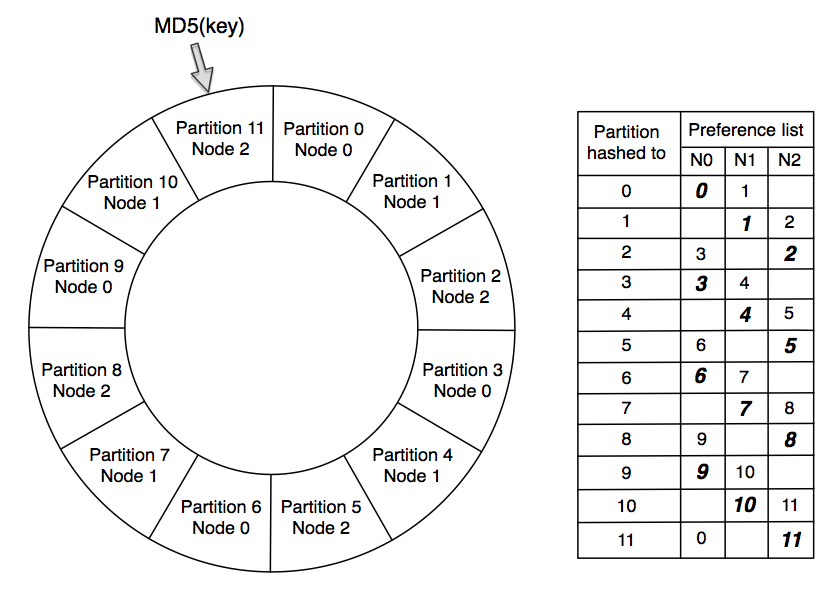
\includegraphics[width=0.5\textwidth]{introduction/hashring_voldemort}
    \caption{Hash ring with 3 nodes and 12 partitions from Voldemort\cite{dynamo} with N=2. Partitions are a fixed number of splits of the keyspace. Nodes are assigned a number of partitions which they hold. When a request is routed, one first hashes the key to find the partition the key belongs on. One then asks nodes in the order of the \emph{preference list} for the key.}
    \label{fig:voldemort_hashring}
\end{wrapfigure}

To help provide higher availability of data, an optimistic approach to replication is used.
By allowing replicas to gradually propagate in the background and not synchronously, the workload on a distributed database system is greatly relieved, allowing for higher throughput. By also allowing conflicting data, we can continue to serve data in times of failure. This will cause more work for the application developers, and they need to be aware of this when using the database. Allowing conflicts also helps availability of put operations, and allows us the possibility to always accept a write.

It is easy to see how the consistent hashing ring helps implement this approach in Voldemort.
To ensure data durability, one can simply write the data to the next few nodes on the ring. In Dynamo and Voldemort this is a tunable parameter, W, which controls how many nodes a write synchronously has to reach to be successful. 
Internally it is called \emph{required writes}.

Similarly, it is easy to see how we can implement optimistic replication.
By allowing nodes to push written object in the background at a later time to any number of nodes further down the ring.
This number \emph{N}, is called the \emph{replication factor}, and designates the number of replicas we \emph{eventually} want to be present.
I.e. we will have an \emph{eventually consistent} form of replication.


\subsubsection{Conflicts}
To facilitate the high demand for availability, Voldemort and Dynamo always allow writes.

vector clocks

\subsubsection{Membership}
gossip

\subsubsection{Failures}

\subsubsection{Tunability}
The system gives the admin the opportunity to fine tune certain parameters after what the system needs.
These are called N,R,W

\subsection{Goals}
Create a system for automatically including new nodes in a set of member nodes.
For Voldemort, this includes redistributing partitions and updating routing information without making the system unresponsive, ie. without incurring downtime.


